\documentclass{standalone}
\usepackage{tikz}

\newcounter{node}

\begin{document}
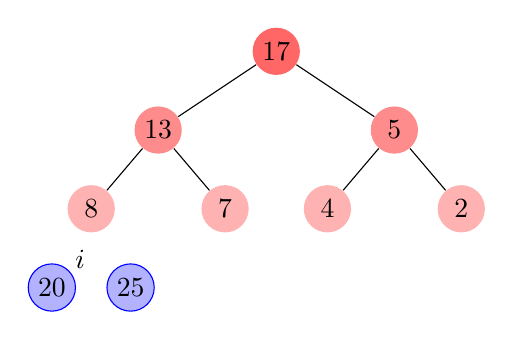
\begin{tikzpicture}
  [level distance=10mm,
    label distance=-3pt,
    every node/.style={fill=red!60,circle,inner sep=1pt, minimum size=6mm},
    level 1/.style={sibling distance=30mm,nodes={fill=red!45}},
    level 2/.style={sibling distance=17mm,nodes={fill=red!30}},
  level 3/.style={sibling distance=10mm,nodes={fill=red!25}},
]

  \node {17}
  child {node {13}
    child {node {8}
      child {node [draw=none, label={45:$i$}, fill=blue!30, draw=blue] {20} edge from parent[draw=none]}
      child {node[draw=none, fill=blue!30, draw=blue] {25} edge from parent[draw=none]}
    }
    child {node {7}
      child[missing] 
      child[missing]
    }
  }
  child {node {5}
    child {node {4}
      child [missing]
    child [missing]
    }
    child {node {2}
        child [missing]
        child [missing]
    }
  };
\end{tikzpicture}
\end{document}





